% !TEX root = Theo_III.tex


\chapter{Elemente der Vektoranalysis\label{elemente_der_vektoranalysis}}

\section{Vektoranalysis}

\subsection{Gradient und Nabla-Operator}

Der Gradient eines skalaren Feldes $U$ ist definiert über das totale Differential:
\begin{equation*}
	\diff U=\grad U\cdot \diff \vec {r}=\nabla U\cdot \diff \vec {r}
\end{equation*}
Der Gradient steht senkrecht auf den Äquipotentiallinien. Für kartesische Koordinaten gilt
\begin{equation*}
	\nabla =\vec {e}_{x}\frac{\partial }{\partial x}+\vec {e}_{y}\frac{\partial }{\partial y}+\vec {e}_{z}\frac{\partial }{\partial z}=\sum _{i}\vec {e}_{i}\nabla _{i},
\end{equation*}
während für krummlinige allgemein gilt, dass
\begin{equation*}
	\nabla =\sum _{i}\vec {e}_{i}\frac{1}{\left| \partial \vec {r}/\partial x_{i}\right| }\frac{\partial }{\partial x_{i}}.
\end{equation*}
\subsection{Divergenz eines Vektorfeldes\label{ref-007}}

Die Divergenz eines Vektorfeldes $\vec {a}$ wird beschrieben durch
\begin{equation*}
	\divg \vec {a}\left(\vec {r}\right)=\nabla \cdot \vec {a}\left(\vec {r}\right).
\end{equation*}
Sie gibt die Quellenhaftigkeit von $\vec {a}$ an. In kartesischen Koordinaten ist $\divg \vec {a}=\sum _{i}\nabla _{i}a_{i}$.



\begin{figure}[htb]
	\centering
	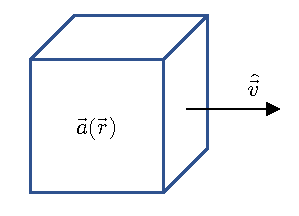
\includegraphics{vecanalysis_flow.pdf}
	\caption{}
	\label{fig:vecanalysis_flow}
\end{figure}

Betrachte zum Verständnis ein kleines Volumen $\Delta  V$ bei $\vec {r}$. Die Normalen $\hat{\vec {\nu }}$ zeigen überall nach außen. Der Fluss aus $\Delta  V$ heraus ist
\begin{equation*}
	q\left(r\right)\Delta  V,
\end{equation*}
wobei $q\left(r\right)=\divg \vec {a}$. Wir können sagen, dass
\begin{align*}
	q\left(\vec {r}\right)=\divg \vec {a}=\begin{cases} >0, & \text{Quelle von }\vec {a}                     \\
              <0, & \text{Senke von }\vec {a}                      \\
              =0, & \text{was reinflie\ss t},\text{flie\ss t raus}
	                                      \end{cases} .
\end{align*}



\subsection{Rotation eines Vektorfeldes}

Die Rotation eines Vektorfeldes $\vec {a}$ ist definiert als
\begin{equation*}
	\rot \vec {a}\left(\vec {r}\right)=\nabla \times \vec {a}\left(\vec {r}\right)
\end{equation*}


\begin{figure}[htb]
	\centering
	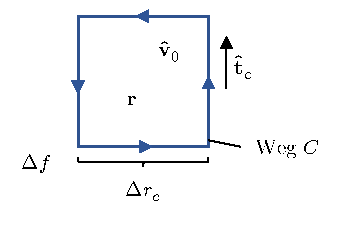
\includegraphics{vecanaylsis_curl.pdf}
	\caption{}
	\label{fig:vecanaylsis_curl}
\end{figure}

und es wird auch als das Wirbelfeld von $\vec {a}$ bezeichnet. Wieder ist die Darstellung in kartesischen Koordinaten einfach: $\left(\rot \vec {a}\right)_{i}=\varepsilon _{ijk}\partial _{{x_{j}}}a_{k}$.

Wir schauen uns ein kleines orientiertes Flächenelement $\Delta  f$ an. Dann ist die Verwirbelung/Zirkulation um $\Delta  f$
\begin{equation*}
	\sum _{C}\vec {a}\cdot \hat{\vec {t}}_{C}\Delta  r_{C}=\rot \vec {a}\cdot \Delta  f
\end{equation*}
mit Tangentialvektor $\hat{\vec {t}}_{C}$ und Parallelkomponente $\vec {a}\cdot \hat{\vec {t}}_{C}$. Wir bezeichnen $\vec {\omega }=\rot \vec {a}$ als lokale Wirbelstärke.

Allgemein gilt, dass Gradientenfelder wirbelfrei sind,
\begin{equation*}
	\vec {a}=\grad U\equivalence \rot \vec {a}=0\quad\mathrm{bzw.}\quad  \rot \left(\grad U\right)=0
\end{equation*}
und Wirbelfelder quellenfrei sind,
\begin{equation*}
	\divg \vec {B}=0\equivalence \vec {B}=\rot \vec {A}\quad\mathrm{bzw.}\quad  \divg \left(\rot \vec {A}\right)=0.
\end{equation*}
Wir definieren ferner den Laplace-Operator als
\begin{equation*}
	\Delta  \equiv \nabla ^{2}\equiv \nabla \cdot \nabla ,
\end{equation*}
für den in kartesischen Koordinaten gilt:
\begin{equation*}
	\nabla ^{2}=\partial _{x}^{2}+\partial _{y}^{2}+\partial _{z}^{2}.
\end{equation*}
\subsection{Fundamentalsatz der Vektoranalysis (Helmholtz-Theorem)\label{ref-009}}

Das Helmholtz-Theorem besagt, dass Quellen und Wirbel ein Vektorfeld $\vec {a}\left(\vec {r}\right)$ eindeutig bestimmen. Ein Vektorfeld kann also in ein Rotationsfeld und ein Wirbelfeld aufgeteilt werden:
\begin{equation*}
	\vec {a}=\underset{\substack{
			\omega =\rot \vec {a}=\rot \vec {a}_{t} \\
			\divg \vec {a}_{t}=0 \\
			\text{Wirbel}!
		}}{\underbrace{\vec {a}_{t}}}+\underset{\substack{
			\rho =\divg \vec {a}=\divg \vec {a}_{l} \\
			\rot \vec {a}_{l}=0                     \\
			\text{Quellen}!
		}}{\underbrace{\vec {a}_{l}}}+\underset{\substack{
			\rot \vec {a}_{r}=\divg \vec {a}_{r}=0 \\
			\text{Randbedingungen}                 \\
			\hat{\vec {\nu }}\cdot \vec {a}=f\left(\vec {r}\right),\vec {r}\in \partial V
		}}{\underbrace{\vec {a}_{r}}}
\end{equation*}
Eine zusätzliche, sowohl quellen- als auch wirbelfreie Komponente kann vorkommen, um Randbedingungen zu erfüllen oder einen konstanten Untergrund zu addieren.

Ebene Transversalwellen ($e^{i\vec {k}\cdot \vec {r}}\perp \vec {k}$) sind zum Beispiel quellenfrei, ebene Longitudinalwellen ($e^{i\vec {k}\cdot \vec {r}}\parallel \vec {k}$) sind dagegen wirbelfrei, denn
\begin{equation*}
	\divg \left(e^{i\vec {k}\cdot \vec {r}}\right)=i\vec {k}\cdot e^{i\vec {k}\cdot \vec {r}},\quad \rot \left(e^{i\vec {k}\cdot \vec {r}}\right)=i\vec {k}\times e^{i\vec {k}\cdot \vec {r}}.
\end{equation*}




\section{Integration von Feldern}


\subsection{Linienintegrale}


\begin{equation*}
	\int _{C}\vec {a}\left(\vec {r}\right)\cdot \diff \vec {r}=\int _{C}\vec {a}\left(\vec {r}\left(s\right)\right)\cdot \frac{\diff \vec {r}}{\diff s}\diff s
\end{equation*}


\begin{figure}[htb]
	\centering
	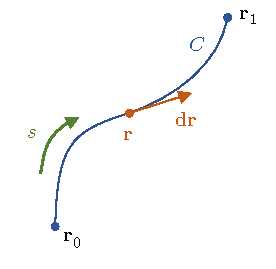
\includegraphics{vecanaylsis_curve.pdf}
	\caption{}
	\label{fig:vecanaylsis_curve}
\end{figure}

Parameterdarstellung: $\vec {r}=\vec {r}\left(s\right)\rightarrow \diff \vec {r}=\frac{\diff \vec {r}}{\diff s}\diff s$ mit der Bogenlänge $s$.

Für rotationsfreie (Einschränkung, siehe Satz von Poincaré) Felder ist das Linienintegral zwischen zwei Punkten wegunabhängig:
\begin{equation*}
	\oint \vec {a}\cdot \diff \vec {r}=0\equivalence \vec {a}\left(\vec {r}\right)=\nabla \varphi \equivalence \rot \vec {a}=\vec {0}.
\end{equation*}


\subsection{Satz von Stokes}

\begin{equation*}
	\underset{\text{Fluss von }\rot \vec {a}~\text{durch} F}{\underbrace{ \int _{F}\rot \vec {a}\cdot \diff f}}=\underset{\text{Zirkulation von }\vec {a}~\text{entlang}~ C=\partial F}{\underbrace{\oint _{C=\partial F}\vec {a}\cdot \diff \vec {r}}}
\end{equation*}

\begin{figure}[htb]
	\centering
	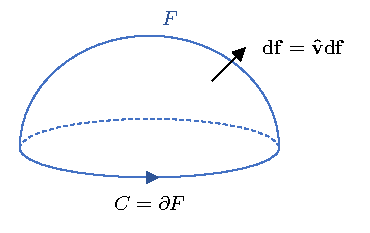
\includegraphics{vecanaylsis_normal.pdf}
	\caption{}
	\label{fig:vecanaylsis_normal}
\end{figure}

Die Kurve $C$ ist dabei stets so orientiert, dass sie der Rechte-Hand-Regel folgt. Von außen (die Seite, nach der der Normalenvektor $\diff \vec {f}$ zeigt) betrachtet geht die Kurve gegen den Uhrzeigersinn.


\subsection{Satz von Gauß}

\begin{equation*}
	\underset{\text{Quellen von }\vec {a}~\mathrm{in} V}{\underbrace{ \int _{V}\divg \vec {a}\cdot \mathrm{dV}}}=\underset{\substack{
			\text{Fluss von }\vec {a}~\text{durch } \\
			\partial V \mathrm{aus}~V \text{heraus}
		}}{\underbrace{\int _{\partial V}\vec {a}\cdot \diff f}}
\end{equation*}
Aus den Satz von Gauß abgeleiteten Formen:
\begin{itemize}
	\item $\vec {a}=g\vec {e}_{i}\rightarrow \int _{V}\frac{\partial }{\partial x_{i}}g\diff V=\int _{\partial V}g\diff f_{i}$

	\item $g=a_{j}\rightarrow \int _{V}\rot \vec {a}\diff V=\int _{\partial V}\diff \vec {f}\times \vec {a}$

	\item Greensche Identitäten (diese finden ihre Anwendung in der Potentialtheorie, hierzu wird $\nabla ^{2}\varphi $ verwendet). $\vec {a}_{1}=\varphi \nabla \psi , \vec {a}_{2}=\psi \nabla \varphi $.

	      \begin{enumerate}[a]
		      \setcounter{enumii}{14}

		      \item[o] 1. Identität: $\int \nabla \cdot \vec {a}_{1}\diff V$
			      \begin{equation*}
				      \int _{V}\left(\nabla \varphi \cdot \nabla \psi +\varphi \nabla ^{2}\psi \right)\diff V=\int _{\partial V}\varphi \nabla \psi \cdot \diff f
			      \end{equation*}
		      \item[o] 2. Identität: $\int \left(\nabla \cdot \vec {a}_{1}-\nabla \cdot \vec {a}_{2}\right)\diff V$ (Greenscher Satz)
			      \begin{equation*}
				      \int _{V}\left(\varphi \nabla ^{2}\psi -\psi \nabla ^{2}\varphi \right)\diff V=\int _{\partial V}\left(\varphi \nabla \psi -\psi \nabla \varphi \right)\cdot \diff f
			      \end{equation*}
	      \end{enumerate}
\end{itemize}
